\chapter{文献综述}
\subsection{欠膨胀射流的流场结构与测量研究}
国内外在轴对称自由欠膨胀射流（静止介质中）领域已积累大量系统性研究成果，相关核心研究通过实验观测、理论推导与数值模拟，从射流形成机制、结构特征、参数规律到建模方法形成了完整研究体系。
Shapiro在1953年通过可压缩流体热力学的系统性分析\supercite{shapiro1954dynamics}，首次明确了欠膨胀射流的本质定义与形成的热力学基础。其研究以收敛喷嘴为核心对象，通过构建纵向压力演化模型，详细分析了流体从喷嘴内部到出口外部的压力变化规律。实验中，他通过控制流体总压与环境压力的比值，观察到两种关键流动状态：当总压比未达到临界值时，流体出口压力与环境压力平衡，流速处于亚声速；当总压比达到临界值后，喷嘴进入壅塞状态，出口流速达到声速，此时出口压力仍高于环境压力，流体无法在喷嘴内部完成压力平衡，只能在出口外部通过激波结构调整压力，进而形成欠膨胀射流。该研究还通过热力学方程推导，验证了壅塞状态是欠膨胀射流形成的前提这一核心结论，其提出的压力比临界判定逻辑，成为后续各类射流类型判定的基础框架。
Courant等人从超声速流动与激波理论出发\supercite{courant1948formation}，深入阐释了欠膨胀射流形成的物理本质。他们通过激波动力学分析，指出流体在出口处的压力失衡是形成欠膨胀射流的核心驱动力，而外部激波的产生是流体向环境压力平衡的必然热力学过程。研究中，他们采用特征线法对超声速流动进行数值求解，模拟了激波在射流中的产生、传播与反射过程，验证了激波结构是流体压力调整的关键载体这一结论。此外，他们还通过实验观测到激波与射流边界的相互作用，明确了激波强度与压力比的正相关关系，为射流结构的研究奠定了理论基础，其提出的激波分析方法被广泛应用于超声速射流的数值模拟。
Abramovich通过大量射流实验与理论推导\supercite{abramovich1963theory}，提出射流沿轴向分为近场、过渡、远场三区域的经典框架，该框架目前仍是射流结构分析的核心依据。其研究以空气为工作介质，采用热线风速仪、压力传感器等设备，系统测量了不同压力比下射流的速度、压力、温度分布。在近场区域，他发现核心区流体与环境流体几乎无交换，主要经历等熵膨胀与激波压缩，流速保持超声速；混合层则由湍流主导，存在明显的速度梯度，通过大尺度涡结构实现流体动量交换，且混合层中存在超声速与亚声速两个子区域，以恒定压力线为分界。过渡区域中，他观测到压力、温度等参数的变化率显著降低，射流与环境流体充分混合，压力场逐渐趋于均匀，混合层厚度持续增加并向轴线靠近。远场区域中，射流完全膨胀，流动呈现自相似性，轴向速度和温度随距离增加呈双曲线衰减，径向分布符合高斯分布特征，且该区域的流动特性与理想膨胀射流高度相似。
Islam通过不同压力比下的对比实验\supercite{islam2024theoretical}，系统分析了压力比对射流区域结构的影响。他采用收敛喷嘴，工作介质涵盖空气、氮气、氩气，压力比范围为1~10，通过纹影法可视化射流结构，结合压力传感器测量关键截面压力。实验发现，低压力比（1~1.1）下，近场仅存在单一正激波，射流结构简单，过渡区与远场的划分距离较短；中压力比（1.1~4）下，近场形成复杂的激波胞结构，激波与膨胀波交替出现，过渡区长度显著增加；高压力比（$\ge$7）下，激波胞数量减少，仅存单个主激波胞，马赫盘呈弯曲状，远场自相似性的建立距离大幅延长。此外，他还发现流体性质对区域结构的影响较小，而喷嘴出口几何（如喷嘴角）会改变近场激波的反射方式，进而影响区域划分。该研究量化了压力比对射流区域结构的影响规律，为不同压力比场景下的射流预测提供了实验数据支撑。
Crist等人通过大规模实验\supercite{crist1966study}，系统研究了喷嘴下马赫盘位置的规律。实验中，他们采用轮廓喷嘴与锥形喷嘴，工作介质为空气，总压力比范围覆盖2~1000，出口直径为0.5~2.0~mm，通过纹影法定位马赫盘位置，结合压力传感器验证压力分布。通过对大量实验数据的拟合分析，他们提出马赫盘位置与总压力比的关联规律：总压力比越大，马赫盘距离喷嘴出口越远，且该规律在宽压力比范围内均适用，预测误差小于10\%。此外，他们还发现马赫盘位置与流体性质（如比热容比）无关，与喷嘴出口直径呈线性比例关系，提出了实用的马赫盘位置估算方法。
部分研究聚焦马赫盘直径的定量规律\supercite{addy1981effects,murugesan2020numerical}，通过对比实验分析了喷嘴几何、压力比、流体性质对马赫盘直径的影响。实验中，研究者采用轮廓喷嘴、锥形喷嘴与孔道三种出口形式，工作介质为空气、氢气、氮气，总压力比范围为5~100。低压力比（5~50）下，轮廓喷嘴的马赫盘直径大于锥形喷嘴，且两者均随压力比增大而增大，研究者提出了针对性的关联式；高压力比（$\ge$50）下，马赫盘直径与马赫盘位置的比值趋于常数，收敛喷嘴的常数为0.6，直喷或扩张喷嘴的常数为0.4。此外，马赫盘直径与流体比热容比呈反比，氢气的马赫盘直径仅为空气的60\%左右。该研究量化了喷嘴几何与流体性质对马赫盘直径的影响，但实验数据离散度较大，需进一步验证。
Phalnikar等人聚焦微喷嘴（出口内径$<$1~mm）的激波胞特征，补充了微尺度下的射流规律\supercite{phalnikar2008experiments}。实验中，他们采用出口直径为0.1~0.9~mm的微喷嘴，工作介质为空气，压力比范围5~20，通过显微纹影法可视化激波结构，结合微型压力传感器测量压力分布。实验发现，微尺度下超声速核心长度显著缩短，仅为宏观喷嘴的五分之一至三分之一，且激波胞的衰减速度更快；激波胞尺寸与喷嘴出口直径呈线性比例关系，微喷嘴的激波胞尺寸显著小于宏观喷嘴；粘性效应在微尺度下更为显著，导致激波胞的强度衰减更快，混合层厚度占射流直径的比例更大。
Palmer与Hanson早期采用特征线法进行射流建模\supercite{phalnikar2008experiments}，该方法是射流核心区激波结构预测的经典数值方法。其核心原理是将复杂的可压缩流动控制方程分解为易于求解的常微分方程，沿特征线方向积分求解，能准确捕捉激波的产生与传播。研究中，他们针对振动非平衡流动场景，模拟了欠膨胀射流核心区的激波结构，验证了特征线法在非平衡流动中的适用性。结果表明，该方法能准确预测马赫盘位置、激波强度分布，误差小于8\%，适用于火箭发动机喷管出口激波结构、超声速燃烧器入口射流等场景的流场分析。但该方法存在局限：对混合层湍流效应的描述能力有限，难以准确捕捉湍流引发的复杂混合过程，且计算效率较低，不适用于全流场（近场+远场）的模拟。
Dash等人基于Navier-Stokes方程开发简化数值模型\supercite{dash1978analysis}，该模型通过忽略横向粘性扩散，将三维流动问题简化为二维抛物型方程，适用于射流轴向参数演化的快速预测。实验验证中，他们以空气为工作介质，压力比范围5~20，模拟了射流轴向速度、压力的演化规律，与实验数据的误差小于10\%。该模型的核心优势在于计算效率高，仅为传统Navier-Stokes方程求解的1/5，适用于工程初步设计、多工况参数扫描等场景。但由于简化假设的存在，该模型对径向混合效应的模拟精度有限。
Khaksarfard等人在2010年通过氢气射流模拟\supercite{khaksarfard2010numerical}，揭示了理想气体模型在高压场景下的局限性，强调了真实气体模型的必要性。氢气在高压下（总压力比大于50），分子间作用力不可忽略，压缩因子偏离1，理想气体模型预测的密度与声速误差超过20\%。研究中，他们采用范德华方程和Peng-Robinson方程两种真实气体模型，模拟了压力比50~200下的氢气射流热力学行为，与实验数据对比表明，修正后的密度与声速预测误差可降至5\%以内。此外，他们还发现高压下氢气的比热容比随压力变化显著，理想气体模型假设比热容比恒定会进一步放大误差。
Mohamed与Paraschivoiu进一步验证了真实气体模型在超临界流体射流中的适用性\supercite{mohamed2005real}。超临界流体（如高压二氧化碳）的热力学行为与理想气体差异极大，理想气体模型无法描述其相变前的状态。研究中，他们以超临界二氧化碳为工作介质，压力比范围100~400，采用Peng-Robinson方程模拟射流的热力学演化，实验中通过激光拉曼光谱测量密度与温度分布。结果表明，Peng-Robinson方程能准确捕捉超临界流体从超临界到亚临界的过渡过程，密度预测误差小于8\%，而理想气体模型的误差超过50\%。该研究将真实气体模型的应用范围扩展至超临界流体，填补了超临界射流建模的空白。
Otobe等人观察到湿空气射流中的冷凝现象，揭示了相变对射流结构的影响\supercite{kim2009effect}。湿空气在膨胀过程中温度和压力骤降，可能进入亚稳态引发冷凝，这一现象会改变射流的热力学性质和流动结构。实验中，他们以湿空气为工作介质，相对湿度范围30\%~80\%，压力比范围5~30，通过高速摄影技术捕捉冷凝过程，结合压力传感器测量马赫盘特征。结果发现，冷凝会导致马赫盘直径减小10\%~15\%，且马赫盘位置出现滞后现象——压力升高与降低时，马赫盘位置不同，这一现象与冷凝过程的非瞬时性密切相关。
Baek等人补充了冷凝对射流结构的定量影响\supercite{baek2006study}，进一步完善了相变射流的理论。实验中，他们以不同湿度的湿空气为工作介质，压力比范围10~40，通过纹影法可视化激波结构，测量冷凝对激波胞、混合层的影响。结果表明，冷凝对射流结构的影响随湿度增大而增强：相对湿度从30\%增至80\%时，马赫盘直径减小幅度从10\%增至15\%，激波胞波长缩短幅度从12\%增至18\%；在RESS（超临界溶液快速膨胀）过程中，固体颗粒的析出会使马赫盘位置缩短20\%，曲率增大。该研究量化了湿度与相变程度对射流结构的影响，为含水汽相变射流的精准预测提供了实验数据。
Bülent在2002年测试欠膨胀超声速射流的射流扩张特性及中心线参数衰减规律\supercite{yuceil2002scaling}，确定了一组合适的归一化参数，该参数需能够表征射流的初始膨胀过程，并支持在大跨度出口-环境压力比范围内，对射流的渐近混合速率开展横向对比。实验采用专用探针完成数据采集，该探针可同步测量射流流场中的当地总压、静压、总温以及环境背景参数。测试区域覆盖射流的亚声速段，部分工况下的测量距离最远可达喷管出口截面的270倍喷管直径。最后，基于新提出的归一化参数对实验结果进行分析，明确了射流的渐近特性参数规律。
上述实验为研究欠膨胀射流的特性提供了充足的支撑，而在CFD仿真方面也有许多与实验相类别的结果\supercite{gibbons2023eilmer,jin2021nsfnets}。2023年Duronio等人围绕射流特性的实验诊断方法与计算流体力学数值模拟技术展开论述\supercite{duronio2023under}，先考察了工程中常用的喷射参数，再梳理了喷管近场区域的流动特征，最后探讨了对油气混合形成过程具有显著影响的射流远场湍流混合机制。类似对于典型欠膨胀射流的研究有很多，在2015年Franquet等人的这篇综述作为该领域的总结性文献\supercite{franquet2015free}，汇总了该领域关键实验研究的核心信息，明确了各研究的喷嘴参数、主要测量对象及核心发现，为后续近场区域特征的深入分析与交叉验证提供基础，具体内容可以参考表\ref{tab:jet_review}。
\begin{longtable}{p{3.2cm} p{3.4cm} p{3.2cm} p{4.5cm}}
	\caption{欠膨胀射流实验研究总结}
	\label{tab:jet_review} \\
	\toprule
	研究团队/年份 & 喷嘴参数 & 已测参数 & 核心结论 \\
	\midrule
	\endfirsthead
	\multicolumn{4}{c}{续表：\ref{tab:jet_review} 欠膨胀射流实验研究总结} \\
	\toprule
	研究团队/年份 & 喷嘴参数 & 已测参数 & 核心结论 \\
	\midrule
	\endhead
	\bottomrule
	\endfoot
	\bottomrule
	\endlastfoot
	Crist et al. (1966) & 收敛喷嘴（轮廓/锥形），出口直径0.5~2.0~mm & 马赫盘位置、马赫盘直径、激波胞结构、压力分布 & 1. 马赫盘位置与$P_0$成正比，关联式适用宽压力比；2. 高压力比下马赫盘直径/位置趋于常数（收敛喷嘴0.6）；3. 流体比热容比与马赫盘直径呈反比 \\
	Addy (1981) & 轮廓喷嘴、锥形喷嘴、孔道，出口直径未明确 & 马赫盘直径、喷嘴几何影响、不同流体对比 & 1. 低压力比下轮廓喷嘴马赫盘直径大于锥形喷嘴，均随压力比增大而增大；2. 收敛喷嘴喷嘴角增大，马赫盘直径减小；3. 氢气马赫盘直径仅为空气的60\% \\
	Antsupov (1974) & 收敛喷嘴、收敛-扩张喷嘴，喷嘴角5$^\circ$\~30$^\circ$ & 马赫盘形成临界条件、激波胞类型、喷嘴角影响 & 1. 马赫盘出现临界喷嘴角$\beta_{SR}=\arctan(0.22\sqrt{M_e-1})$；2. 出口马赫数、比热容比增大，马赫盘形成压力比范围拓宽；3. 按出口压比划分弱/中/强/极强欠膨胀激波胞形态 \\
	Love et al. (1959) & 收敛喷嘴，出口直径0.8~1.2~mm & 第一激波胞长度、马赫盘特征、喷嘴几何影响 & 1. 第一激波胞长度随出口压比、出口马赫数增大而增加；2. 提出第一激波胞长度经验公式；3. 喷嘴几何对激波胞结构影响显著 \\
	Ashkenas \& Sherman (1964) & 收敛-扩张喷嘴，出口马赫数$M_e=1.0\sim3.0$ & 马赫盘位置、超声速出口适配性、比热容比影响 & 1. 超声速出口时，马赫盘位置随出口马赫数增大而显著增加；2. 提出含出口马赫数、比热容比、出口压力比的修正关联式；3. 适用于收敛-扩张喷嘴超声速欠膨胀场景 \\
	Avduevskii et al. (1970) & 收敛喷嘴，出口直径1.0~mm & 激波胞结构、粘性效应影响、混合层对激波胞的作用 & 1. 弱欠膨胀（出口压比1~1.1）为出口正激波，中度欠膨胀（1.1~3）为菱形激波胞；2. 粘性效应导致激波胞强度沿下游衰减；3. 混合层增厚加速激波胞瓦解 \\
	Phalnikar et al. (2008) & 微喷嘴（出口直径0.1~0.9~mm） & 激波胞长度、超声速核心长度、微尺度粘性效应 & 1. 微喷嘴超声速核心长度仅为宏观喷嘴的1/5~1/3；2. 激波胞衰减速度快于宏观喷嘴；3. 粘性效应主导微尺度射流激波结构 \\
	Wilcox et al. (1957) & 收敛喷嘴，未明确具体尺寸 & 马赫盘位置、激波胞数量与分布、喷嘴边界层粗糙度影响 & 1. 马赫盘位置随总压比增大而线性增加；2. 不同压力比下激波胞数量与波长存在显著差异；3. 喷嘴边界层粗糙度影响激波胞对称性 \\
\end{longtable}
\subsection{激光测量技术}
当前针对超声速射流的非侵入式诊断技术虽已在流场动力学特性研究中获得诸多应用，但都难以适配欠膨胀射流中CO$_2$相变及热力学参数的精准测量需求。激光诱导荧光（PLIF）在CO$_2$欠膨胀射流冷流工况中，流场无天然荧光活性物质，必须人工掺入甲苯等荧光示踪剂\supercite{lee2021}，而示踪剂与CO$_2$的密度、粘度等物性差异显著，会破坏流场热力学平衡，干扰CO$_2$的快速膨胀过程与相变触发条件，导致测量结果偏离真实场景。即使在低粒子负载的两相流中，示踪剂仍会通过影响相间传热与动量交换，间接改变相变演化路径，这一干扰在超声速冷流工况下更为突出\supercite{bonnin2022}。
2023年Rodrigues等人的研究\supercite{rodrigues2023}，整合了高光谱分辨率激光诱导荧光（NO-PLIF）技术在可压缩流多参数测量中的实验设计与数据处理经验，选用NO分子在226~nm附近的两组相邻吸收线对，通过脉冲模式激光与光学参量振荡器（OPO）系统优化，实现100~kHz高重复率测量，激光线宽窄至0.015~cm$^{-1}$以捕捉流动诱导的碰撞位移信号，还提出了核心数据处理方案：提取峰位与振幅，结合流场轴对称特性分离碰撞位移与多普勒位移分量和双线转动测温法（基于玻尔兹曼分布模型，利用两组线对振幅比反演温度），为温度、压力、速度的同步测量奠定基础；实验成功捕捉到欠膨胀射流的流场结构与参数分布特征，与流场物理规律吻合，但定量测量面临挑战：100~kHz重复率下激光片能量分布的逐次波动导致荧光光谱散射，快速频率扫描的步长不确定性影响峰位定位精度，高温高压区域的激光吸收与荧光饱和效应也会干扰测量准确性。
\begin{figure}[H]
	\centering
	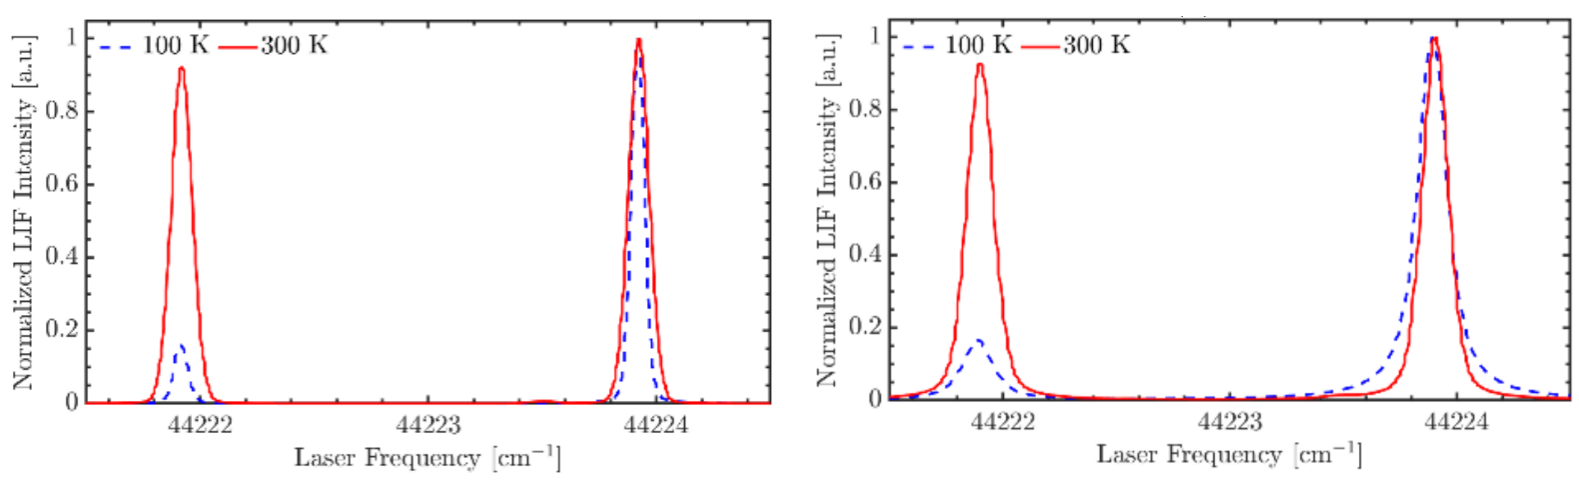
\includegraphics[width=0.8\textwidth]{figures/fig1.png}
	\caption{使用LIFBASE模拟的归一化激光诱导荧光（LIF）强度与激光频率的关系，温度分别为100~K和300~K，压力对应三种不同情况，其中包括1~kPa和10~kPa。}
	\label{fig:lif_sim}
\end{figure}
\begin{figure}[H]
	\centering
	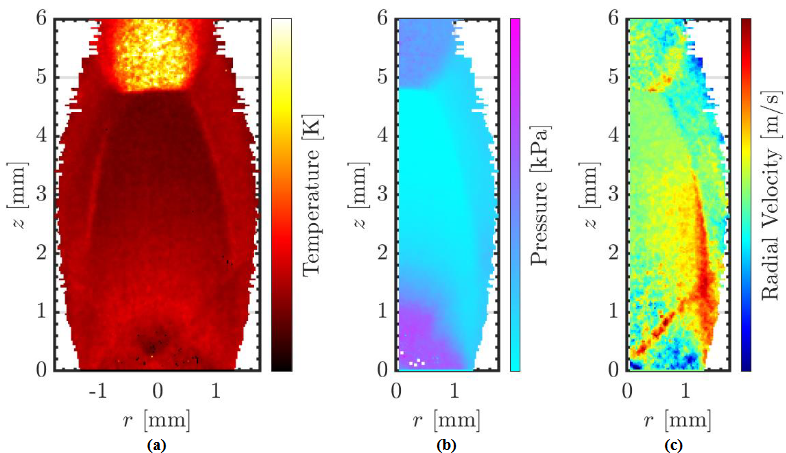
\includegraphics[width=0.8\textwidth]{figures/fig2.png}
	\caption{实验构建的（a）二维温度场（b）二维压力场（c）二维径向速度场}
	\label{fig:lif_exp}
\end{figure}
粒子图像测速（PIV）依赖播撒外部粒子\supercite{samimy2000}，而超声速流场对示踪粒子的松弛特性要求极高，现有粒子的惯性无法跟随高速流场的瞬时变化，易导致速度测量出现显著滞后误差\supercite{williams2015}。该技术仅能获取速度场信息，无法直测温度、压力、密度等相变关键参数，间接推导过程需依赖理想气体状态方程等不合理假设，而CO$_2$相变过程中偏离理想气体行为的特性会进一步放大误差。在液态CO$_2$释放形成的气固两相射流中，外部粒子还会与CO$_2$相变产生的固体颗粒碰撞融合，改变相变产物的分散规律与冷却机制，严重干扰相变演化的真实过程。
纹影法虽无示踪剂需求、完全非侵入，但仅能通过密度梯度引起的光线偏折定性观察激波形态\supercite{hirschberg2002}，无法定量输出热力学参数，难以建立相变现象与温压密等核心参数的量化关联，无法为相变机制解析提供关键数据支撑。
在光谱学领域，分子束光谱技术是一种经典的研究手段。该技术通常通过超声速膨胀射流，将高压混合气体经微米级喷嘴绝热膨胀至高真空环境中，形成一束高度冷却、准直且内部碰撞频率极低的分子束\supercite{jansen2024}。在此过程中，分子的平动温度可降至数开尔文以下，转动和振动自由度也得到显著冷却，使分子多处于基态振转能级，大幅减少多普勒展宽和碰撞展宽对光谱线型的影响，光谱分辨率可达兆赫兹甚至亚兆赫兹量级，非常适用于分子精细结构、超精细能级及微弱光谱信号的探测。然而，该技术虽然在基础分子光谱研究中具有不可替代的优势，但其应用场景存在明显局限：通常要求目标分子处于静止且孤立的高真空束流状态，需通过磁光阱、缓冲气体冷却等技术实现分子的深度冷却与捕获，完全脱离工程实际中CO$_2$欠膨胀射流的常压/低压、高密度碰撞环境；且该技术仅将射流当作分子束的产生源，并未关注射流本身的激波结构、混合演化等关键特征，因此无法真实反映原始流场中参数的时空演变及相变与流动的耦合机制。
中红外激光光谱测量技术凭借非侵入式、高灵敏度、快速响应的特性，以及无需添加示踪剂即可直接探测气体特征吸收谱线的优势，已成为流场参数测量的重要手段。其工作原理将激光调谐至目标物种（如H$_2$O、CO$_2$、CO）不同振转量子态的近邻跃迁，通过测量吸收光谱推断粒子数比，进而计算温度；测量至少2条谱线，即可获取目标物种的摩尔浓度。国内外在该技术用于复杂工况的参数测量领域已积累长期且系统的成果\supercite{zapryagaev2018}，例如2020年Wen等人的研究\supercite{wen2020}，该研究整合了光谱测量技术在非接触诊断中的实验方法与数据处理经验，选择CO$_2$在4.2~$\mu$m附近的特征吸收谱线，通过光学系统优化将探测光束直径缩减至150~$\mu$m，以匹配轴对称特性的梯度特征\supercite{yan2023}，还提出了两种核心数据处理方法：高光谱断层扫描技术（结合Abel反演解决视线积分非均匀性误差）\supercite{hickstein2019}和多线谱拟合方法（基于Boltzmann分布模型描述参数径向分布），两种方法的交叉验证提升了测量可靠性；温度测量范围极广且与数值模拟结果吻合良好，但发现CO$_2$浓度测量在高温火焰中误差较高，主要受拟合算法对温度的敏感性影响，瞬态测量虽通过信号滤波实现0.2~ms时间分辨率，但原始信号噪声仍会影响结果稳定性。
2018年Zhang等人的研究同样是光谱测量技术的准确应用\supercite{zhang2018}，通过反演算法创新与实验验证，进一步提升了光谱测量技术在含噪声实际场景中的可靠性。该研究针对性解决了传统光谱测量技术在轴对称测量中的核心痛点——Abel反演算法对实验噪声敏感、重建精度不足的问题。此前，其他研究虽已将洋葱剥离法、三点插值法等用于Abel反演，但这些方法在处理离散测量数据和噪声时，易出现误差累积，尤其在测量的中心区域精度下滑。Zhang等人创新采用傅里叶分析Abel反演算法，通过将衰减系数展开为余弦函数叠加，实现了天然的低通滤波效果，无需额外预处理即可有效抑制噪声。数值模拟验证显示，在1\%噪声条件下，该算法对温度和CO$_2$浓度的重建误差仅为传统洋葱剥离法的$1/3\sim1/4$，尤其在轴对称中心和边缘区域，重建结果更贴合真实分布，大幅提升了复杂场景下的测量稳定性。类似的还有Marakasov的研究团队\supercite{marakasov2023}在俄罗斯西伯利亚分院理论与应用力学研究所的立式射流实验装置上，基于激光透射法的实验测量结果，对超声速射流内空气平均密度的空间分布特征展开分析，对基于透射波前横向（沿射流轴线垂直方向）偏移反演空气平均密度的算法进行了实验验证。随后，将密度反演结果与已发表文献中的接触式测量数据，以及数值模拟结果进行了对比验证。实验结果表明，局部波前倾斜量对离散声频下的空气密度振荡具备良好的敏感性。这一发现为开展射流流道内空气密度不均匀性空间结构的实验研究提供了可行路径。
总体而言，以上研究为本课题提供了可靠的红外光谱测量方法支撑：其验证的CO$_2$~4.2~$\mu$m适配谱段、优化的Abel反演与噪声抑制算法、成熟的温度校准方案，为解决本课题超声速射流CO$_2$相变测量中抗干扰、高精度、非侵入的核心需求，精准捕捉热力学参数、解析相变机制提供了关键技术保障。
\subsection{相变机制研究}
国内外CO$_2$相变研究围绕“欠膨胀射流动态相变”展开，形成“实验可视化--理论建模--数据验证”的完整体系，核心聚焦成核、生长、蒸发全流程的机制解析。其中经典成核理论（Classical Nucleation Theory, CNT）是理解相变初始阶段，特别是从亚稳态母相中产生新相晶核过程的基石性理论框架\supercite{oxtoby1992}，其理论根源可追溯至Gibbs在19世纪末对界面热力学的奠基性工作，其中引入的“吉布斯自由能变化”概念，首次明确了相变需要克服一个临界能垒。20世纪上半叶，经过Volmer、Weber、Becker与Döring等学者的系统发展，CNT从热力学和动力学两个维度得以完善\supercite{becker1935}。从热力学角度看，CNT将新相核（如液滴或晶体）视为具有宏观界面性质的球形簇，其形成过程中的吉布斯自由能变化是体积自由能下降与表面自由能增加相互竞争的结果。1962年的热力学研究明确了包含$n$个分子的液滴形成过程中吉布斯自由能变化与临界半径的关联，揭示了过饱和度对临界液滴尺寸的调控规律\supercite{mcdonald1963}；1963年的动力学研究则建立了成核速率的定量计算方法，补充了分子簇生长与分解的速率方程，为后续相变机制解析提供了核心理论支撑，实现了从微观分子聚集行为到宏观相变速率的桥接，为相变过程的预测提供了关键理论工具。尽管CNT在解释许多宏观相变现象上取得了巨大成功，但其理论局限性也随着研究深入而不断显现\supercite{baek2006study}。其核心假设——将纳米尺度的分子簇视为具有块体材料热力学性质（如界面张力）的宏观液滴——在描述极小核或复杂分子系统时面临挑战。这促使了更为精细的理论与模拟方法的发展，如密度泛函理论（DFT）和分子动力学（MD）模拟，它们能够从分子层面揭示成核的微观机制，同时，针对不同应用场景的修正CNT模型也相继提出，例如考虑温度梯度、非等温效应、多组分耦合以及非经典成核路径的拓展理论\supercite{cnt2006}。在此基础上，Harding于1965年首次将完善后的CNT与可压缩流体等熵膨胀方程耦合\supercite{harding1965}，开发出全球首个针对单组分流体快速膨胀凝结过程的数字化计算程序，该文献基于经典成核理论（CNT）构建了单组分蒸汽膨胀凝结的数值计算模型，核心应用于凝结起始点判定、临界液滴参数计算及成核速率求解，适用于单组分蒸汽的快速膨胀流动（如喷管内流动），假设蒸汽膨胀过程中凝结成核遵循热力学平衡准则，临界液滴形成是成核核心判据，液滴生长与成核过程相互独立且分步计算，需输入蒸汽饱和特性、表面张力、潜热等热力学参数，温度范围覆盖蒸汽三相点上下区域，临界液滴半径（$r^*$）是成核的关键参数，基于表面张力与化学势差平衡推导得出，基础公式为：
\begin{equation}
	r^* = \left( \frac{2\mu}{\rho_L RT \ln \frac{p}{p_\infty}} \right) \sigma
\end{equation}
其中，\(\mu\) 为蒸汽分子量，\(\rho_L\) 为液体密度，\(R\) 为通用气体常数，\(T\) 为当地温度，\(p\) 为当地压力，\(p_\infty\) 为饱和蒸汽压，\(\sigma\) 为液滴表面张力。考虑有限液滴尺寸对表面张力的影响，需通过托尔曼（Tolman）修正公式调整表面张力：
\begin{equation}
	\sigma = \frac{\sigma_\infty}{1 + \frac{D}{r}}
\end{equation}
将修正后的表面张力代入临界半径公式，得到简化表达式：
\begin{equation}
	r^* = \left( \frac{2\mu}{\rho_L RT \ln \frac{p}{p_\infty}} \right) \sigma_\infty - D
\end{equation}
式中，\(D\) 为托尔曼常数（经验拟合参数），\(\sigma_\infty\) 为平面液体表面张力。
成核速率（\(J\)）表征单位体积、单位时间内形成的临界液滴数量，基于玻尔兹曼统计力学推导，公式为：
\begin{equation}
	J_T = \left( \frac{p}{kT} \right)^2 \frac{1}{\rho_L} \sqrt{\frac{2\sigma \mu}{\pi N_A}} e^{-\frac{4\pi \sigma r^*}{3kT}}
\end{equation}
其中，\(k\) 为玻尔兹曼常数，\(N_A\) 为阿伏伽德罗常数，指数项为成核自由能垒（由临界液滴的表面能决定），前置项包含蒸汽分子数密度、液滴形成的动力学因子。
凝结起始点的判定遵循特定逻辑：从饱和点开始，以固定温度步长（\(\Delta T \geq 5\ \text{K}\)）进行等熵膨胀迭代；对每个迭代步，计算临界液滴半径 \(r_T^*\) 和成核速率 \(J_T\)，进而得到该步的凝结质量分数增量 \(\Delta g_T\)：
\begin{equation}
	\Delta g_T = \frac{4\pi \rho_L}{3\dot{m}} \dot{N}_T {r_T^*}^3
\end{equation}
随后通过压力/温度偏差系数判断凝结是否显著，亚声速流动采用压力偏差系数：
\begin{equation}
	\epsilon_p = \frac{A}{\Delta A} \left( \frac{L}{C_p T} - 1 \right) \Delta g_T
\end{equation}
超声速流动采用温度偏差系数：
\begin{equation}
	\epsilon_T = \frac{A}{\Delta A} \left[ \left( \frac{\gamma - \frac{1}{M^2}}{\gamma - 1} \right) \frac{L}{C_p T} - 1 \right] \Delta g_T
\end{equation}
当 \(\epsilon\) 达到设定临界值（\(\epsilon_{\text{critical}}\)）时，判定为凝结起始点，输出该点的压力、温度、位置等参数。
该程序采用密歇根算法解码器（MAD）语言编写，适配IBM 7090大型计算机，可通过自定义喷嘴几何、初始工况等参数，定量预测凝结起始位置、液滴生长速率及流场温压演化，其凝结起始点搜索-流场与相变迭代耦合的核心框架，为后续相变数值模拟奠定了基础。2021年Wu等人研究欠膨胀射流中纯\(\text{CO}_2\)及\(\text{CO}_2\)-空气混合物的相变行为\supercite{wu2021}，直接继承并拓展了这两项成果：一方面，其构建的准一维膨胀流模型沿用了Harding的流场-相变耦合逻辑，仅将单组分分压修正为\(\text{CO}_2\)-\(\text{N}_2\)双组分分压，以适配混合工质场景，且Harding程序较好的预测的单组分\(\text{CO}_2\)凝结起始位置（\(z/D \approx 0.1\)）。首次采用单脉冲、高重复率（250~kHz）二维瑞利散射成像技术，实现\(\text{CO}_2\)团簇相变全流程可视化与定量测量。关键发现：①成核起始于喷嘴出口近场（\(z/D=0.1\sim0.4\)），初始临界团簇半径约3.7~nm，受过饱和度调控快速收缩至0.4\(\sim\)0.6~nm并稳定；②马赫盘（\(z/D=2.1\)）后因温压骤升，团簇在\(1\mu\text{s}\)内快速蒸发，散射强度下降一个数量级；③\(\text{CO}_2\)摩尔分数降低（从100\%至7\%）会显著抑制成核（成核速率下降60\%以上），高出口压力（\(P_e=200\ \text{psig}\)）可强化团簇形成；④相变过程未显著改变射流的桶形激波与马赫盘结构，仅局部影响剪切层混合。Li于2010年发表的研究\supercite{li2009}，以Ramos et al.（2005）通过Rayleigh与Raman散射测得的\(\text{CO}_2\)团簇尺寸、数密度等实验数据为基准，构建了兼具均相和非均相凝结过程的\(\text{CO}_2\)凝结羽流模型，创新采用基于直接模拟蒙特卡洛（DSMC）的凝结模型框架，不仅精准复现了低滞止压力下纯\(\text{CO}_2\)均相凝结流动的特性，还针对5\%\(\text{CO}_2\)与95\%\(\text{N}_2\)混合工质的膨胀流动，开发了\(\text{N}_2\)分子在\(\text{CO}_2\)核上凝结的动力学模型，系统考虑了液滴团聚效应对相变过程的影响——这一改进有效弥补了传统模型在高过饱和度场景下的预测缺陷，显著提升了成核速率计算的精度，其模拟的瑞利散射强度与实验数据也达成良好吻合。该模型“结合工质组分特性、耦合均相-非均相凝结机制、量化液滴团聚影响”的核心建模思路，为后续动态流场中\(\text{CO}_2\)团簇演化的计算提供了重要参考。2024年Wagner等人针对高速分散多相流中湍流、激波与颗粒相互作用的复杂机制及模拟实验挑战\supercite{capecelatro2024}，围绕亚声速至超声速工况下的气-固颗粒相互作用开展系统性综述研究。梳理了与马赫数相关的阻力定律发展脉络，而颗粒分辨数值模拟技术为该定律的优化完善提供了全新视角；从单颗粒层面切入，系统归纳了单颗粒运动方程及相关现象学规律，明确了可压缩两相流区别于不可压缩多相流的核心运动尺度特征；针对多颗粒系统，从数值模拟与实验测试双维度，剖析了涵盖含尘气体至稠密悬浮液的多类多颗粒体系流动特性，为高速多相流的工程应用与理论研究搭建了系统化的知识框架。
\begin{figure}[H]
	\centering
	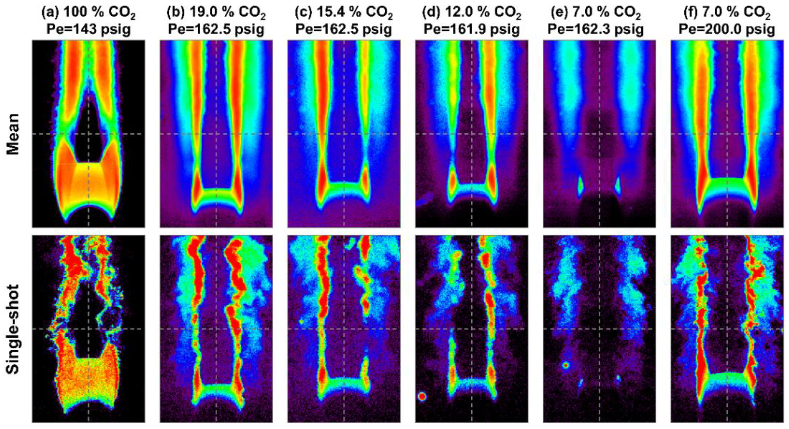
\includegraphics[width=0.8\textwidth]{figures/fig3.png}
	\caption{纯二氧化碳及二氧化碳-空气混合射流中二氧化碳团簇的瑞利成像}
	\label{fig:rayleigh}
\end{figure}
\begin{figure}[H]
	\centering
	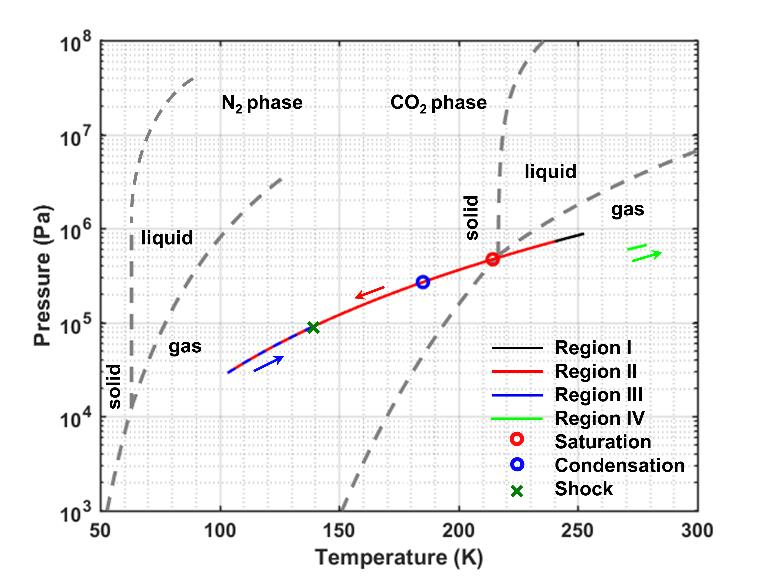
\includegraphics[width=0.8\textwidth]{figures/fig4.png}
	\caption{CO$_2$在欠膨胀超声速射流中的温压演化轨迹与相变状态的对应关系}
	\label{fig:pt_path}
\end{figure}
2025年侯佳鑫等人针对跨声速低温风洞非接触式测量的示踪粒子短缺难题\supercite{hou2024}，建立Laval喷管中氮气非平衡凝结的多相流数值模型，结合经典成核理论（CNT）与示踪特性评估方法，系统分析自发凝结氮液滴的生成规律与示踪可行性。确立了氮液滴非平衡凝结分为快速成核区与液滴生长区，成核需\(5.5\,\text{K}\)过冷度（Wilson点），液滴数量由成核区凝结核决定，粒径由生长区生长速度控制，可独立调控；自发凝结氮液滴粒径\(0.5\sim7\,\mu\text{m}\)范围内，Stokes数为\(10^{-3}\)量级，在马赫数\(0.5\sim1.5\)（速度\(94\sim282\,\text{m/s}\)）下随流性优良，满足示踪要求；液滴生成时间约\(75\,\mu\text{s}\)，小于其响应时间，可在凝结过程中完成速度调整，快速跟随气流运动，准确反映流场真实速度；不同粒径液滴示踪时长适配各类低温风洞：\(1\,\mu\text{m}\)粒径可运动\(2.1\,\text{m}\)，\(7\,\mu\text{m}\)粒径可运动\(106.4\,\text{m}\)，分别适配\(0.3\,\text{m}\) TCT风洞（需\(1\sim10\,\text{m}\)）与\(2.5\,\text{m}\) NTF风洞（需\(100\,\text{m}\)）。
2019年Deng等人针对Laval喷管内两种典型可凝结工质（水汽、\(\text{CO}_2\)）\supercite{deng2019}，通过数值模拟结合相变理论，系统探究其在喷管流动中的凝结与膨胀协同演化规律。发现两种工质凝结起始位置存在显著差异，\(\text{CO}_2\)的凝结起始点更靠近喷嘴喉部，水汽则在扩张段中后程启动凝结，根源是两者饱和热力学特性与膨胀过程中温压演化速率的不同；凝结释放的潜热会反向影响流场特性，会使\(\text{CO}_2\)流场的膨胀速率降低\(15\%\sim20\%\)，水汽流场的压力恢复幅度提升\(10\%\)左右，体现相变与流场的强耦合效应；\(\text{CO}_2\)的成核速率峰值是水汽的\(2\sim3\)倍，但液滴生长速率更低，最终形成的液滴粒径比水汽小\(30\%\sim40\%\)，反映工质物性对相变全流程的调控作用；喷嘴扩张角对\(\text{CO}_2\)相变影响显著，当扩张角从\(5^\circ\)增至\(15^\circ\)时，\(\text{CO}_2\)凝结区域向出口方向移动，液滴数量密度下降\(25\%\)以上，为喷管结构优化提供关键依据。
尽管现有研究取得了一定进展，但仍存在三个关键缺口：其一，理论模型与动态流场实际工况脱节，现有相变理论多基于静态假设，难以描述欠膨胀射流中激波反射、湍流混合与相变成核、液滴生长的耦合机制，真实气体状态方程的适配性不足；其二，实验测量技术存在局限，缺乏能同时满足“非接触干扰、全域覆盖、多参数同步、高时空分辨”的测量方案，无法精准捕捉相变触发与演化的动态过程；其三，理论与实验的协同验证不足，数值模拟结果缺乏高精度实验数据的支撑，难以有效指导工程实践。本课题正是基于此基础提出，为解决上述问题提供有效地解决方案。
	% ==================== 第三章 Fluent仿真与硬件系统 ====================

